\section{A case study -- using VICE}
\label{sec:viceorg}

The case study presented in this section is used to analyse the performance
of a distributed in-car radio navigation system. The case study was originally
modelled using the Modular Performance Analysis technique, as described in the
paper \textit{``System Architecture Evaluation Using Modular Performance
Analysis -- A Case Study''} by Wandeler et al \cite{orgcase}.
We refer to this paper\footnote{Available at
\textit{http://www.cs.ru.nl/research/reports/info/ICIS-R05005.html}.
Additional information can be found at
\textit{http://people.ee.ethz.ch/$\sim$leiden05/data/pset/p2.pdf}
and at \textit{http://www.mpa.ethz.ch} .} 
for a full description of the case study. 

\begin{figure}[!htb]
\begin{centering}
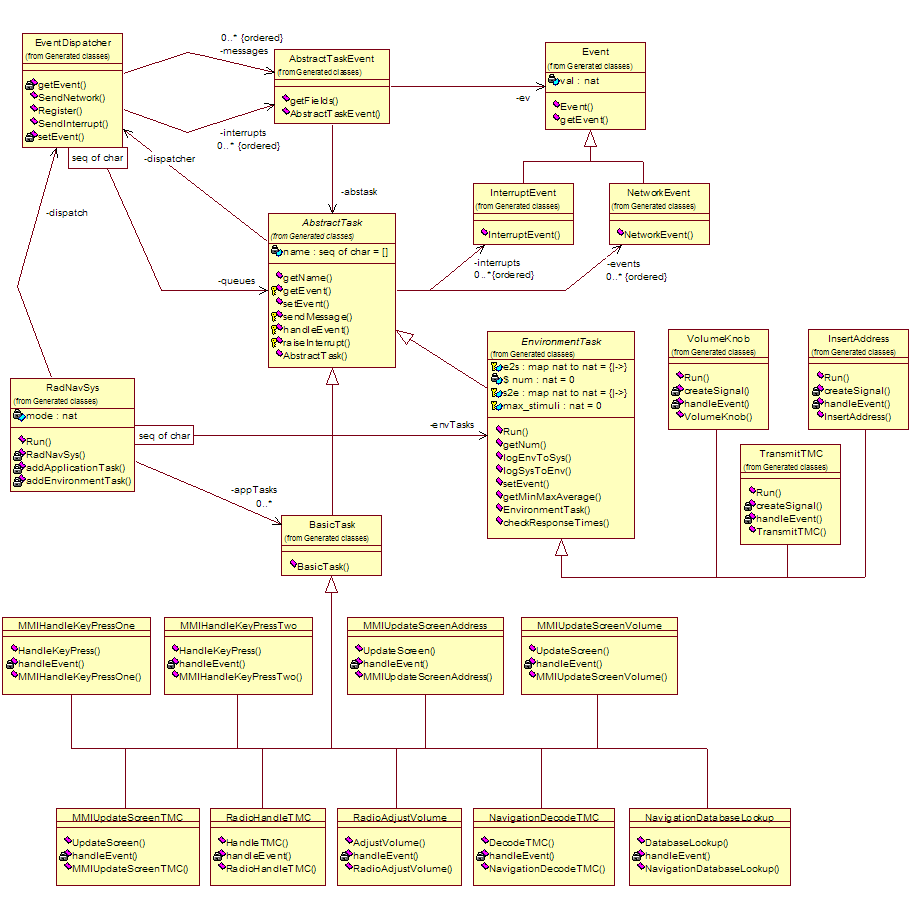
\includegraphics[width=0.8\textwidth]{classold.png}
\caption{UML class diagram of the case study using standard VICE}
\label{fig:uml1}
\end{centering}
\end{figure}

In this note, an attempt was made to describe the same case study using
VDM++, first with the original VICE language and later we will present the
proposed extensions to the language. A UML class diagram of the case study
using the existing VICE technology is shown in Figure~\ref{fig:uml1}.
In Figure~\ref{fig:uml2}, a class diagram of the same case study is shown,
but then using the suggested improvements to the VICE language. It is
immediately clear from those two diagrams that the suggested improvements
significantly reduce the size of the model. But more importantly,
the model using the languages extensions describes the system in
far more detail than the standard VICE specification. The latter can
only describe the single CPU architecture case (and already with some
difficulty because the environment tasks are not really running in
parallel to the embedded system) while the former is able to describe
\textit{all} possible distributed architectures describe in
\cite{orgcase}. Note that our discussions with the CSK team have
already led to changes in the VICE tool. For example, the \verb+time+
keyword was added which allows the user to access the simulation wall
clock of the interpreter directly.

\begin{figure}[!htb]
\begin{centering}
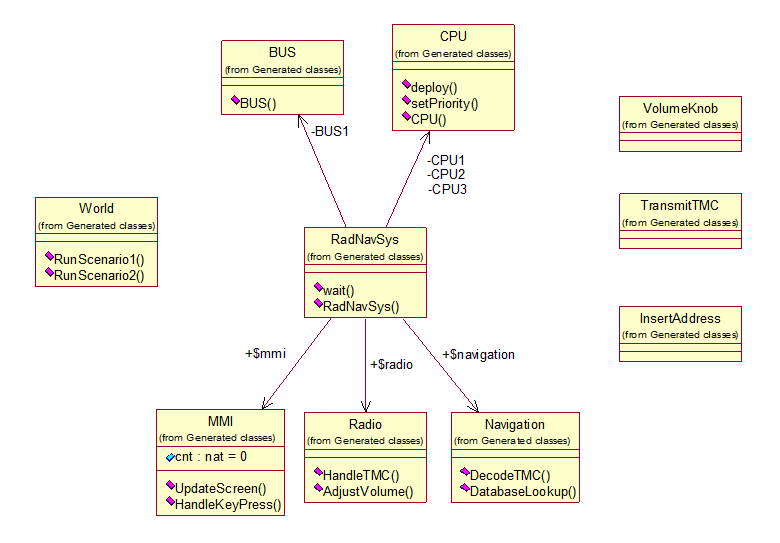
\includegraphics[width=0.6\textwidth]{classnew.png}
\caption{UML class diagram of the case study using the improved VICE notation}
\label{fig:uml2}
\end{centering}
\end{figure}

The in-car radio navigation system is basically a soft real-time system that
executes several concurrent applications at the same time (each consisting
of several tasks), for example for controlling the radio while Traffic Message
Channel data is being processed. Timing requirements are typically specified
per application and the question of interest is whether or not these
requirements are met under all operating conditions, when deployed on
a given architecture. In this note we will consider the situation where all
applications are running on a single CPU, because it is the only configuration
that we can effectively describe using the existing VICE technology. VICE only
supports uni-processor multitasking models, while some architectures considered
in the paper above require a notion of multi-processor multitasking. First, we
will present the model in the existing VICE notation.
In Section~\ref{sec:vicenew} we will present the model
in the improved VICE notation.

\subsection{A mini-framework for reactive systems modelling}

The in-car radio navigation system is a typical real-time embedded system;
it is waiting for stimuli from the environment and processes those events
accordingly. Some stimuli only change the internal system state but most
will cause a response back to the environment. In our case study all
stimuli will cause an external visible response.

Timeliness requirements are often specified in terms of the elapse time
between the stimulus and the response of the system. Such a system is
typically described by an event loop; the system is waiting for stimuli
and when one arrives, it is identified and the appropriate operation is
called and the event loop is immediately resumed. For this to work in
real-time systems, the operation calls shall be asynchronous because
the event loop should never be blocked by the call because it would
potentially delay a high priority event that arrived just after the
event that is currently being processed. Since neither VDM++ nor
VICE supports asynchronous operation calls, we have to mimic this
behaviour by using threads and explicitly describing the event loop.

The Event class is the abstract base class for the events that are managed
by such an event loop. A natural number is used to ``trace'' each individual
event through the system, such that we can specify timing (and temporal)
requirements easily.

\input{Event.vpp.tex}

Two different event types are modelled here: interrupt and network events.
Interrupts are used to trigger the system from the environment, network
events are used to model inter task communication within the system.
As we will see later, interrupts \textit{have priority} over network events.

\input{InterruptEvent.vpp.tex}

\input{NetworkEvent.vpp.tex}

The \verb+AbstractTask+ class provides the basic functionality to handle
events. Two separate input queues are maintained, one for interrupts and
one for network events. There will be a single \verb+EventDispatcher+
instance that will dispatch all system events to the appropriate active
object. The EventDispatcher can raise interrupts or send network events
by calling the public \verb+setEvent+ operation of the applicable
\verb+AbstractTask+ instance. The operations \verb+getEvent+ and 
\verb+handleEvent+ are used to implement the event loop, as we will
see later. Note that \verb+getEvent+ gives priority to interrupts over
network events; calls to the operation will be blocked (because of the
synchronisation predicate) until there is at least one event available.
The \verb+AbstractTask+ can send messages (or raise interrupts) to other
\verb+AbstractTask+s by calling \verb+sendMessage+ or \verb+raiseInterrupt+.
In both cases, the dispatcher will be called to route the message to the
receiving task without blocking the caller.

\input{AbstractTask.vpp.tex}

The \verb+BasicTask+ class implements the event loop. It is an active
object (with its own thread of control) that is constantly processes
incoming events. The task will be blocked when no events are available,
due to the synchronisation predicate specified in the base class.

\input{BasicTask.vpp.tex}

The \verb+EnvironmentTask+ class is used to model tasks in the environment,
outside the scope of the system. EnvironmentTask instances generate the
stimuli for the system and observe the responses coming back. Both stimuli
and responses are administered using the \verb+logEnvToSys+ and 
\verb+logSysToEnv+ operations respectively. The function
\verb+checkResponseTimes+ is used to check the system timeliness
requirements. We will see later how it is used. The operation \verb+getNum+
is used to create unique identifiers, one for each stimulus that is
generated and inserted into the system. Recent discussions with the CSK
team has led to a change in the existing VICE tool already. The \verb+time+
keyword was added to refer to the simulation wall clock of the interpreter.
This feature is used in the \verb+logEnvToSys+ and \verb+logSysToEnv+
operations.

\input{EnvironmentTask.vpp.tex}

\subsection{Modelling the system application tasks}

In this section, the application tasks are listed. There are six tasks
in total. The event loop for each task is simple; the appropriate
synchronous function is called and the next task in the sequence is
signalled by sending a message to it. Note that the time penalty of the
synchronous operation is modelled using the standard VICE duration
statement. First the \verb+MMIHandleKeyPressOne+ class which is used in
scenario~1.

\input{MMIHandleKeyPressOne.vpp.tex}

\noindent Next, the \verb+MMIHandleKeyPressTwo+ class which is used in
scenario~2.

\input{MMIHandleKeyPressTwo.vpp.tex}

\noindent The class \verb+MMIUpdateScreenVolume+ is used in scenario~1
to handle screen updates caused by the volume changes of the radio.

\input{MMIUpdateScreenVolume.vpp.tex}

\noindent The class \verb+MMIUpdateScreenAddress+ is used in scenario~2
to handle screen updates caused by the address lookup actions in the database.

\input{MMIUpdateScreenAddress.vpp.tex}

\noindent The class \verb+MMIUpdateScreenTMC+ is used in both scenarios
to display decoded TMC messages on the screen.

\input{MMIUpdateScreenTMC.vpp.tex}

\noindent The class \verb+RadioAdjustVolume+ is used to adjust the volume
of the radio.

\input{RadioAdjustVolume.vpp.tex}

\noindent The class \verb+RadioHandleTMC+ is used to process incoming TMC
messages over the radio.

\input{RadioHandleTMC.vpp.tex}

\noindent The class \verb+NavigationDatabaseLookup+ is used to search for
an address in the navigation database.

\input{NavigationDatabaseLookup.vpp.tex}

\noindent The class \verb+NavigationDecodeTMC+ is used to decode TMC messages
into a human readable format using the information from the database.

\input{NavigationDecodeTMC.vpp.tex}

\subsection{Modelling the environment tasks}

There are three environment tasks for our case study. One to insert ``key
press'' events (\verb+VolumeKnob+), one to insert ``lookup address'' events
(\verb+InsertAddress+) and one to insert Traffic Message Channel messages
(\verb+TransmitTMC+). The environment inserts these events into the system
by raising an interrupt. Note that all environment tasks exhibit the same
basic structure. The operation \verb+createSignal+ is called periodically
by its own the thread of control to generate the stimulus. Note that we
\textit{have to} use the statement \verb+duration (0)+ explicitly in order
to ensure that the execution of the environment task does not influence
the notion of time of the application tasks in the system model. As a
consequence, we cannot write environment tasks that make use of the
duration statement, for example to insert a second stimulus after
\textit{x} time units, because that would influence the notion of time
of the system model (which is supposed to run in parallel with its ``own''
notion of time). This makes life for the specifier rather difficult in
some cases. The underlying problem is that the uni-processor multitasking
semantics of VICE is \textit{not strong enough} to model both the environment
and the system operating at the same time. We need to move from the
interleaving semantics to true parallel behaviour to describe this properly,
effectively implementing a multi-processor multitasking approach where the
environment task is assigned its own independent processor. \\

Despite this deficiency in VICE, we are still able to express timeliness
properties, as can be seen in the \verb+handleEvent+ operation. Whenever
a response is observed, it is added to the trace information and the
post-condition of the \verb+handleEvent+ operation states that the time
difference between each pair of stimuli and responses shall be less than
some (user-defined) value. Note that there is no completeness requirement
specified here, we can in fact insert more stimuli than we receive back
from the system. This is left out on purpose here; it cannot be checked
on-line because a stimulus might be ``inside'' the system for a very long
time and we are never sure that we waited long enough (this is called the
quiescence property), unless we specify an explicit time-out value for each
expected response. In this specification it is solved by limiting the number
of inserted stimuli and waiting for all responses of all inserted stimuli.
Since the number of stimuli is limited, we know that eventually the system
has enough time to deal with each one. Typically, these kinds of completeness
requirements are processed off-line, after the simulation run is completed;
similarly for temporal properties enforcing some fixed (partial) order in
the stimuli. Another reason for off-line processing might be simulation
efficiency, since the log will increase in size the longer we simulate and
therefore checking the post-condition every time might take up too much
time. When doing post-processing the timeliness, completeness and temporal
requirements only have to be checked once for the trace which makes it
very efficient. \\

Furthermore, we have no explicit control over the start time of the first
period of a periodic task, it is currently dependent on the settings of the
interpreter. This can cause problems because we might know for example that
two otherwise independent environment tasks have the same period but always
run out of phase by some time margin, for example 10 percent of the period.
If the simulator however chooses to activate both periodic tasks right after
one another (remember we use duration zero) that might cause a different
response time behaviour of the system than when the out-of-phase execution
of the environment task was taken into account properly. At the moment,
these kind of problems cannot be handled by the VICE extensions. \\

Another problem is the scheduling of the periodic tasks. Whenever the
periodic task is scheduled, it should become the active task immediately,
pre-empting any other task running, in order to maintain a consistent clock
value. If the periodic task is delayed (or interrupted) by another task that
lets time progress (with some duration greater than zero) then the clock will
become out of sync because we do not know by how much time we were delayed.
If that problem occurs during simulation of the model then the trace files
that are built up here immediately become useless. But more importantly, it
is currently extremely difficult to find out whether or not that problem
actually did occur. So if an invalid trace is detected, is it really an
invalid trace or is it a side-effect of the simulation? \\

\noindent The \verb+VolumeKnob+ class which is used in scenario~1.

\input{VolumeKnob.vpp.tex}

\noindent The \verb+InsertAddress+ class which is used in scenario~2.

\input{InsertAddress.vpp.tex}

\noindent The \verb+TransmitTMC+ class which is used in both scenarios.

\input{TransmitTMC.vpp.tex}

\subsection{Linking everything together -- the event dispatcher}

The EventDispatcher is the most important active object in the specification.
It mediates all the events in the model, both to and from the environment and
to and from the system. Basically, it receives all events, puts them into
temporary queues and greedily dispatches them to the appropriate receivers.
When simulating, the user should ensure that it is the highest priority task
running using pre-emptive scheduling, such that it can process the events
as soon as they become available. The \verb+Logger+ base class is shown in
the appendix. It provides functionality to output the order of the events
that were processed into a file. With the new \verb+time+ keyword it is
now possible to relate this user defined log to the standard log file that
is produced by VICE. Using these two log files in combination can increase
the insight into the model tremendously!

\input{EventDispatcher.vpp.tex}

\subsection{Composing the top-level system model}

The class \verb+RadNavSys+ is the top-level specification for our case-study.
It is used to instantiate and start the model. The system can be analysed
using two different sets of environment tasks exercising the system. The
user can select between the scenarios by supplying the appropriate parameter
to the constructor of the class. For example, the system can be simulated
by calling \verb+new RadNavSys(1).Run()+ on the command-line of VICE.

\input{RadNavSys.vpp.tex}

\subsection{Executing the model}

Before we can execute the model, we have to set up the VICE interpreter.
We use VICE in the pre-emptive scheduling mode, with all options enabled
(dynamic type, invariant, pre- and post-condition checking). The following
task priorities were specified (they are maintained in an external file
called \verb+priority.txt+).

\begin{vpp}
VolumeKnob:10;
InsertAddress:10;
TransmitTMC:9;
EventDispatcher:8;
MMIHandleKeyPressOne:6;
MMIHandleKeyPressTwo:6;
MMIUpdateScreenVolume:5;
MMIUpdateScreenAddress:5;
MMIUpdateScreenTMC:4;
RadioAdjustVolume:3;
RadioHandleTMC:2;
NavigationDecodeTMC:1
\end{vpp}

The environment tasks are given the highest priority, to ensure that they
can indeed inject stimuli whenever their period has expired. Next highest
priority is the \verb+EventDispatcher+ which orchestrates the message
handling between the tasks and the environment. Following are the
application tasks, with priorities as specified in the case study
definition. We can now execute the model using the VICE interpreter.

\begin{vpp}
Initializing specification ...
done
>> priorityfile priority.txt
>> print new RadNavSys(1).Run()
D:/papers/vdmppsem/improve/TransmitTMC.vpp, l. 17, c. 26:
  Run-Time Error 59: The post-condition evaluated to false
>> print e2s, s2e
\{ 1 |-> 2047,3 |-> 3935,4 |-> 4131,6 |-> 5119,8 |-> 6107,10 |-> 7095,
  12 |-> 8083,14 |-> 9071,16 |-> 10059,18 |-> 11047 \}
\{ 1 |-> 25741 \}
\end{vpp}

The VICE interpreter stops in the post-condition of the \verb+TransmitTMC+
operation. We print out the stimuli (e2s) and response (s2e) mappings and
indeed we see that the first stimulus sent actually stayed inside the
system longer than 10000 time units. It is nice that we know that we do
have a problem in our system but can we find the cause of the problem
easily? Actually, that is very hard -- even with the \verb+time+ extension
recently added to VICE. We have to go over the trace files manually, or
use dedicated analysis tools. Even for this simple example the trace file
becomes approximately 300kb, containing several thousands lines of data.
It is clear that powerfull analysis tools are needed to help the user
to better understand the (execution data of the) model.

